The Julia language features a rich ecosystem for scientific computing.
%
LazySets uses \href{https://github.com/JuliaPackaging/Requires.jl}{Requires.jl} to add further functionality depending on whether some external packages are loaded.
%
Here we quickly list various examples, but the list is not exhaustive.
%
From three-dimensional visualizations to reachability analysis using non-convex set representations, there is a broad spectrum of features that are available loading optional dependencies.

\smallskip

Some LazySets functionality prints instructive error messages when the corresponding packages are not loaded but are required by the code. For example, the conversion between constraint and vertex representation of general polytopes in dimension higher than two requires the optional package \href{https://github.com/JuliaPolyhedra/Polyhedra.jl}{Polyhedra.jl}:

\begin{minipage}{\linewidth}
\begin{lstlisting}
julia> X = rand(VPolytope, dim=4)
	
julia> constraints_list(X)
ERROR: AssertionError: package 'Polyhedra' not
  loaded (it is required for executing
  `default_polyhedra_backend`)

# fix the error by loading the optional package
julia> import Polyhedra

julia> constraints_list(X)
12-element Vector{HalfSpace{Float64, ...}}}:
...
	\end{lstlisting}
\end{minipage}


\subsection{Plotting three-dimensional sets and projections}

While writing this article, we received the following question:

\begin{quote}
We need to plot polyhedra given in a form like this:

\begin{center}
	\texttt{2 * x1 >= 0 \& 3 * x2 + 1.7 * x3 >= 0}
\end{center}

Is there a way to plot a 2D projection with LazySets?
\end{quote}

Yes, there is!
We replied with the script below.
The script nicely illustrates the interaction of LazySets with the Julia ecosystem.
We use \href{https://github.com/JuliaSymbolics/Symbolics.jl}{Symbolics.jl} for reading the polyhedron in symbolic form, Polyhedra.jl and \href{https://github.com/JuliaPolyhedra/CDDLib.jl}{CDDLib.jl} for projecting the polyhedron, and \href{https://github.com/JuliaPlots/Plots.jl}{Plots.jl} to plot the two-dimensional projection.

\begin{minipage}{\linewidth}
\begin{lstlisting}
using Symbolics
import Polyhedra, CDDLib, Plots

# projected polyhedron from symbolic constraints
vars = @variables x1, x2, x3  # create symbols
P = HPolyhedron([2*x1>=0, 3*x2+1.7*x3>=0], vars)
Q = project(P, [2, 3])  # 2D projection (x2 and x3)

Plots.plot(Q)  # plot the 2D projection
\end{lstlisting}
\end{minipage}

We can also plot the three-dimensional set with \href{https://github.com/JuliaPlots/Makie.jl}{Makie.jl}.
The Makie plot and the two-dimensional projection are shown in Fig.~\ref{fig:polyhedra}.

\begin{minipage}{\linewidth}
\begin{lstlisting}
import GLMakie

# intersection with a bounding box
B = BallInf(zeros(3), 5.0)
R = intersection(P, B)

plot3d(R)  # plot in three dimensions
\end{lstlisting}
\end{minipage}

\begin{figure}
	\centering
	\hfill
	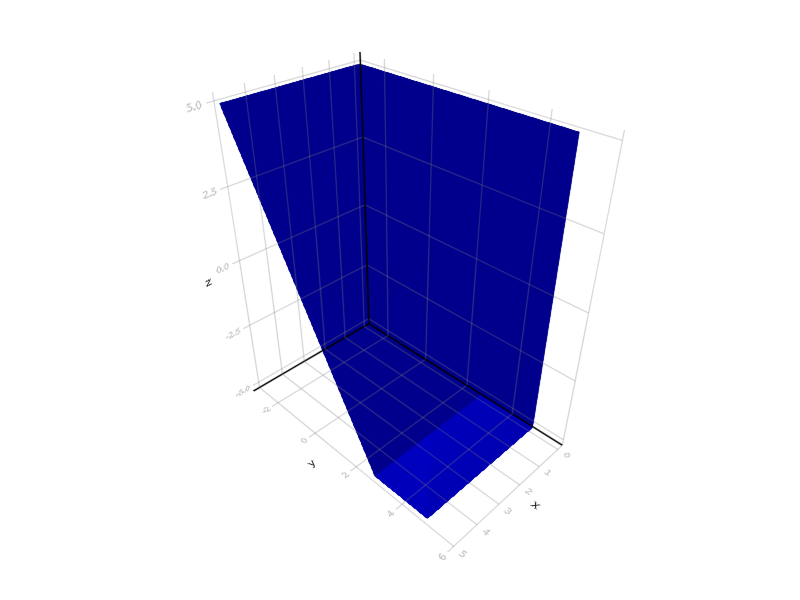
\includegraphics[width=0.49\linewidth, height=3cm, keepaspectratio,clip,trim=65mm 14mm 62mm 19mm]{img/polyhedron3D}
	\hfill
	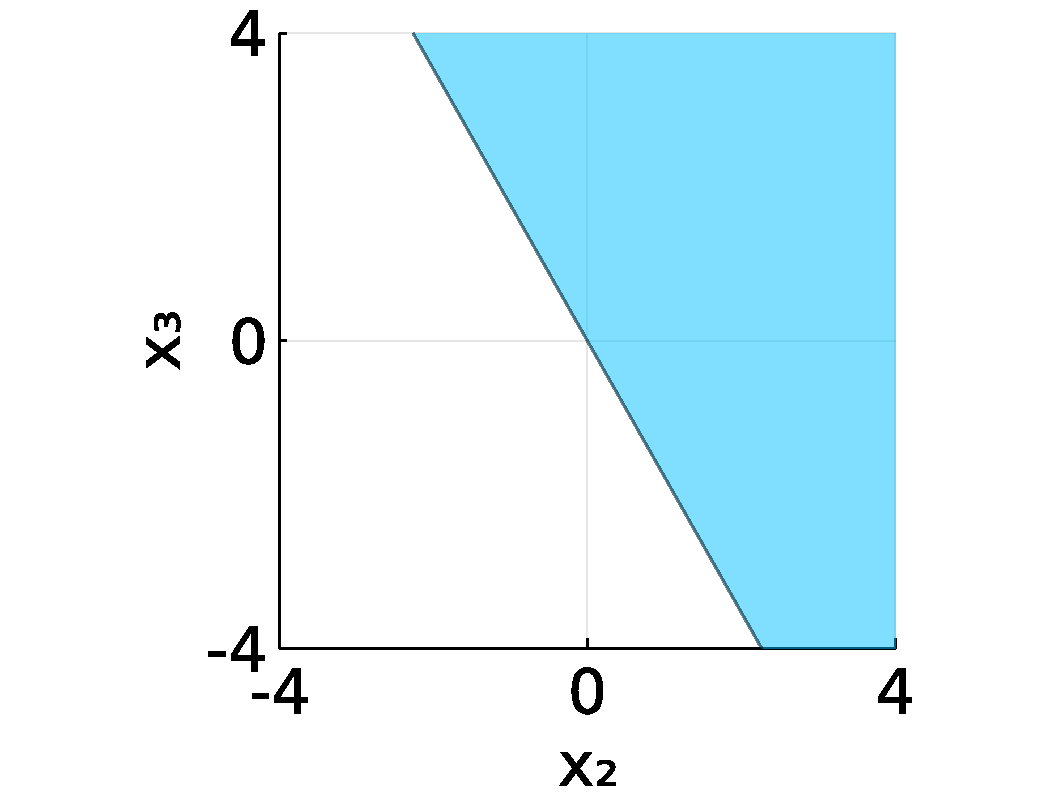
\includegraphics[width=0.49\linewidth, height=3cm, keepaspectratio]{img/polyhedron2D}
	\hfill\,
	\vspace*{1mm}
	\caption{Three-dimensional polyhedron plotted using Makie (left) and a two-dimensional projection obtained by Polyhedra with CDDLib (right).}
	\label{fig:polyhedra}
\end{figure}

\subsection{Generic numbers and automatic differentiation}\label{sec:numbertypes}

LazySets types are parametric in the number type. Hence it is simple to use custom number types.
%
Besides rationals and arbitrary-precision floating-point numbers, it is possible to make rigorous floating-point calculations using \href{https://github.com/JuliaIntervals/IntervalArithmetic.jl}{IntervalArithmetic.jl}.
%
Moreover, LazySets features a mechanism to globally tune the numeric tolerances used in floating-point operations.
%
To do so, use \code{set\_atol}, \code{set\_rtol}, and \code{set\_ztol} (for absolute, relative, and comparison-with-zero tolerance) respectively.
%
All set functions have been carefully designed to consistently use the specified tolerance and preserve it during operations.

\smallskip

Questions from users, bug reports, and feature requests are available in the \href{https://github.com/JuliaReach/LazySets.jl/issues/}{issue tracker}.
%
One question we received was:

\begin{quote}
	Using \href{https://github.com/JuliaDiff/ForwardDiff.jl}{ForwardDiff.jl} to get the gradient of [...] throws the following error:

\texttt{ERROR: default tolerance for numeric type ForwardDiff.Dual\{...\} is not defined}
\end{quote}

The solution was surprisingly simple: extending the LazySets tolerance mechanism to work with dual numbers fixed the error.

\begin{minipage}{\linewidth}
	\begin{lstlisting}
import ForwardDiff
import LazySets.default_tolerance

default_tolerance(::Type{<:ForwardDiff.Dual}) = default_tolerance(Float64)
	\end{lstlisting}
\end{minipage}
With this code, the user could differentiate through the formula \code{area(intersection(X, Y))}, which computes the area of the intersection between sets $\X$ and $\Y$.


\subsection{Taylor models as an example of non-convex sets}\label{sec:taylormodels}

LazySet is not limited to convex set representations. Apart from operating with set unions (\code{UnionSet}), which are generally non-convex, the library offers functionality to handle intrinsically non-convex set representations.
%
Examples include star sets (\code{AbstractStar}), polynomial zonotopes (\code{PolynomialZonotope}), and Taylor models. The latter representation is available in the package \href{https://github.com/JuliaIntervals/TaylorModels.jl}{TaylorModels.jl} \cite{TaylorModels.jl,BenetFSS19}, which LazySets interacts with.

\smallskip

Taylor models are, informally, sets defined by the image of a polynomial map with interval remainders.
%
To illustrate, we consider using LazySets to convert, or evaluate the range, of a Taylor model (the conversion is formally explained in~\cite{schilling2021verification}).
%
It is easy to operate with Taylor models in LazySets (the definition of \code{vTM} for the linear and nonlinear case is given in Appendix~\ref{sec:taylormodels_appendix}):

\begin{minipage}{\linewidth}
	\begin{lstlisting}
using TaylorModels

# approximate a vector of Taylor models
# with a zonotopes
overapproximate(vTM, Zonotope)

# approximate a vector of Taylor models
# with a hyperrectangle
overapproximate(vTM, Hyperrectangle)
	\end{lstlisting}
\end{minipage}

\begin{figure}
	\centering
	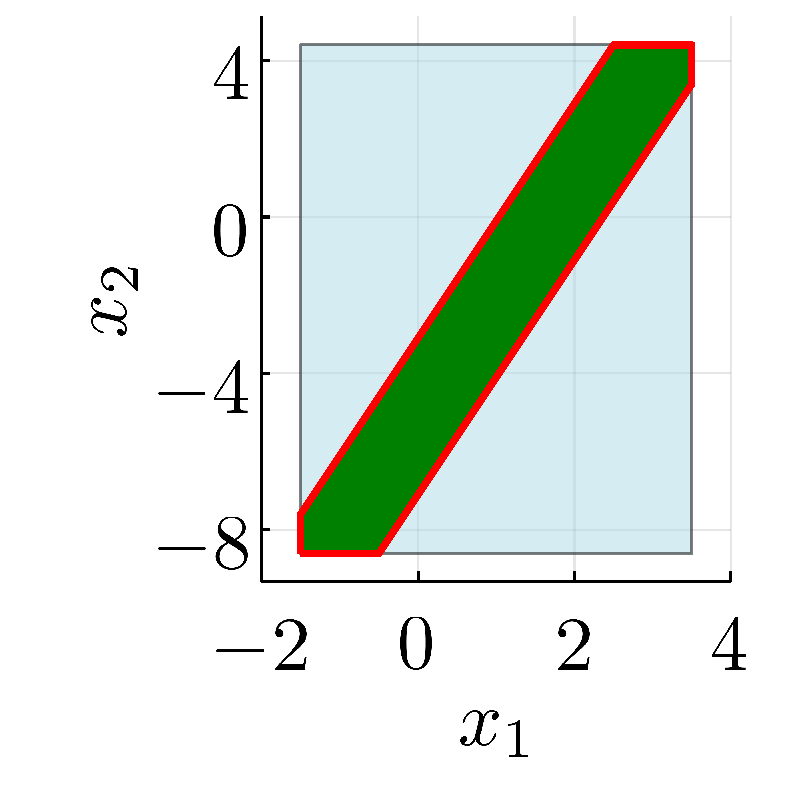
\includegraphics[height=3.5cm, keepaspectratio]{img/taylormodel_linear}
	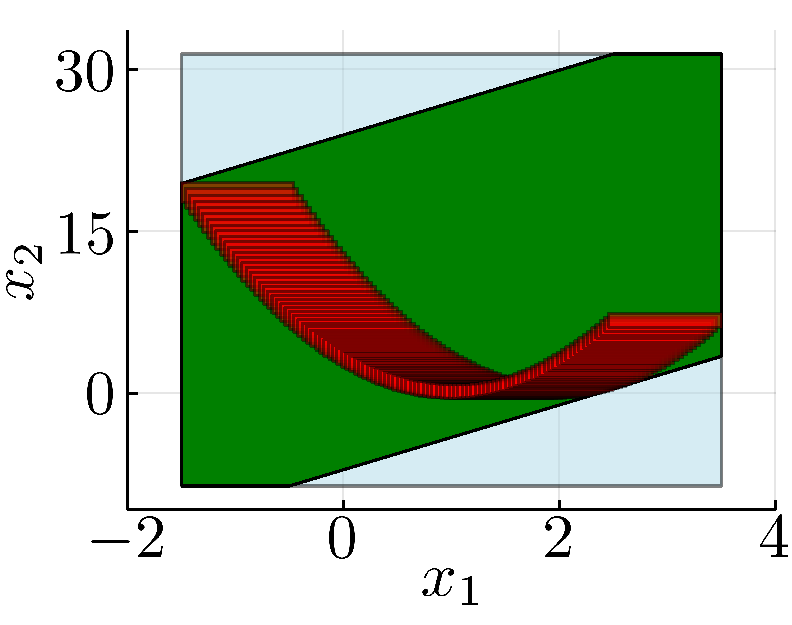
\includegraphics[height=3.5cm, keepaspectratio]{img/taylormodel_nonlinear}
	\caption{Exact conversion of a linear Taylor model to a zonotope against an inexact evaluation using interval arithmetic (left). Approximate conversion of a non-linear Taylor model using a single zonotope, and range evaluation with interval arithmetic by splitting its domain into $100$ intervals (right).}
	\label{fig:taylormodelsconversion}
\end{figure}

In the case when the Taylor model is linear, the conversion is exact, because the zonotope stores linear dependencies between variables.
%
Hence, as is shown in Fig.~\ref{fig:taylormodelsconversion} (left), the zonotope approximation (\code{Z}) is better than directly using interval arithmetic to evaluate the range (\code{H}), and queries about the zonotope provide quick information about the exact set, more accurate than the box approximation:

\begin{minipage}{\linewidth}
	\begin{lstlisting}
julia> d = [-0.35, 0.93]
 
julia> ρ(d, Z)
3.217

julia> ρ(d, H)
4.617000000000001
\end{lstlisting}
\end{minipage}

If the Taylor model contains nonlinear terms, the zonotope provides an enclosure; a comparison against an evaluation using interval arithmetic with many small boxes is shown in Fig.~\ref{fig:taylormodelsconversion} (right).

\smallskip

We also mention that LazySets can be combined with the powerful interval constraint programming approach by simply loading the optional dependency \href{https://github.com/JuliaIntervals/IntervalConstraintProgramming.jl}{IntervalConstraintProgramming.jl}.


\subsection{Reachability applications}

LazySets is the core library of JuliaReach, a Julia ecosystem to perform reachability analysis of dynamical systems.
%
JuliaReach builds on sound scientific approaches and was, in two occasions (2018 and 2020), the winner of the annual friendly competition on Applied Verification for Continuous and Hybrid Systems (\href{https://cps-vo.org/group/ARCH}{ARCH-COMP}).\footnote{JuliaReach also participated in the 2021 edition, but the report is not published yet.}

\smallskip

Reachability techniques are implemented in the JuliaReach package \href{https://github.com/JuliaReach/ReachabilityAnalysis.jl}{ReachabilityAnalysis.jl}, which uses LazySets at its core for dealing with sets, including the computation of flowpipes (union of reachable states).
%
We include two examples. In Fig.~\ref{fig:flowpipe_heli}, a flowpipe for the vertical velocity of an 8-dimensional helicopter model with a 20-dimensional controller from \cite{skogestad2007multivariable} is shown.
%
The model has distributed initial conditions for all variables as well as non-deterministic inputs (input functions can vary arbitrarily within specified bounds).
%
The computation terminates in nearly $50$\,ms, illustrating the precision and speed of LazySets.
%
It should be noted that the set of initial states has $2^{28}$ corner cases, thus even in the simpler setting where the inputs are held constant, exhaustive evaluation using simulations is computationally intractable, since it would require $268$ million runs.

\smallskip
 
As a second example, a three-dimensional flowpipe for the well-known Lorenz system is shown in Fig.~\ref{fig:flowpipe_lorenz}.
%
In this simulation, the initial conditions are defined as a flat hyperrectangle of radius $0.1$ along the $x$ coordinate:

\begin{minipage}{\linewidth}
	\begin{lstlisting}
X0 = Hyperrectangle(low=[0.9, 0.0, 0.0],
				    high=[1.1, 0.0, 0.0])
	\end{lstlisting}
\end{minipage}
%
Reachable states are represented using Taylor models, which are then approximated with zonotopes for further computations.
%
In this case we have exported the LazySets objects to a VTK file using the \href{https://github.com/jipolanco/WriteVTK.jl}{WriteVTK.jl} optional dependency, and the rendering was performed by the open-source visualization tool \href{https://www.paraview.org/}{Paraview}.


\begin{figure}[tb]
	\centering
	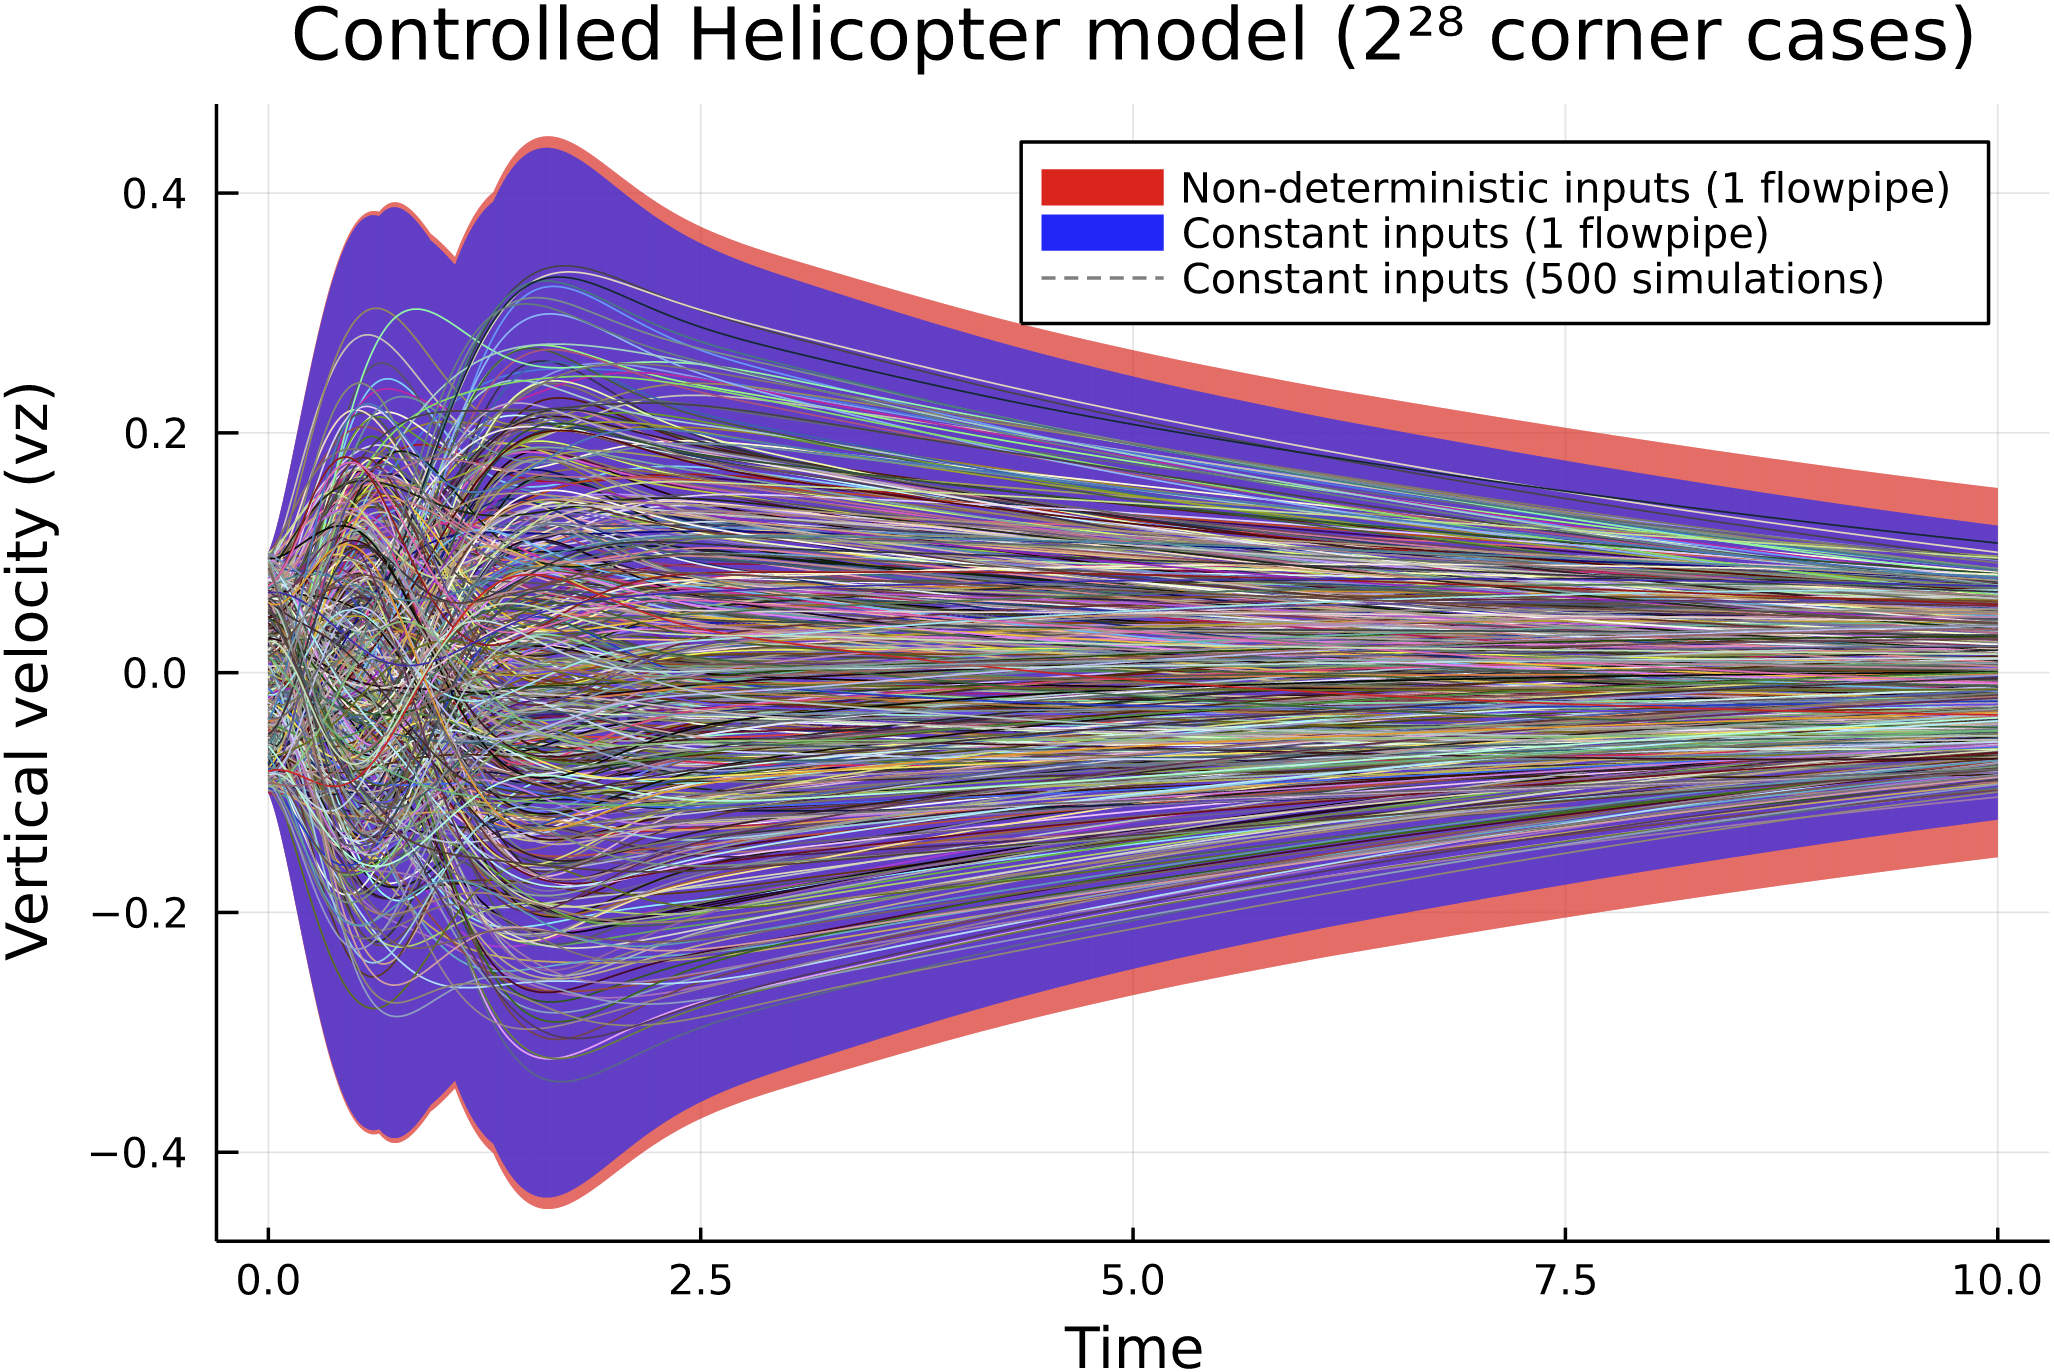
\includegraphics[width=\linewidth,keepaspectratio]{img/heli_08_simu}
	\vspace*{.5mm}
	\caption{Reachable states for the vertical velocity of the helicopter model with non-deterministic inputs. Five hundred trajectories drawn randomly from the set of initial states are shown on top.}
	\label{fig:flowpipe_heli}
\end{figure}

\begin{figure}[tb]
	\centering
	
\includegraphics[width=\linewidth,keepaspectratio,height=4.5cm]{img/lorenz}
	\vspace*{.5mm}
	\caption{Zonotope overapproximation of a Taylor-model flowpipe for the Lorenz equations. The plot is rendered with Paraview.}
	\label{fig:flowpipe_lorenz}
\end{figure}

\subsection{Parametrization and custom array types} \label{sec:custom_arrays}

For set types that contain array fields, we use type parameters. Hence it is possible to instantiate LazySets types with any custom array. Typically, such special arrays (e.g. dense, sparse, static) are used in applications that require high performance.

\smallskip

For example, static arrays (where the size of the array can be determined from the type) are preferable for efficient set computations with ``small'' arrays and are available upon loading \href{https://github.com/JuliaArrays/StaticArrays.jl}{StaticArrays.jl}:

\begin{minipage}{\linewidth}
	\begin{lstlisting}
julia> using StaticArrays

# random ten-dimensional zonotope
julia> Z = rand(Zonotope, dim=10, num_generators=30)

# convert to static arrays
julia> Zs = Zonotope(SVector{10, Float64}(Z.center),
SMatrix{10, 30, Float64}(Z.generators))
julia> d = ones(10)
julia> ds = SVector{10, Float64}(d)

# using normal arrays
julia> @btime ρ($d, $Z)
145.290 ns (0 allocations: 0 bytes)
72.68047192978314

# using static arrays
julia> @btime ρ($ds, $Zs)
44.899 ns (0 allocations: 0 bytes)
72.68047192978314
	\end{lstlisting}
\end{minipage}

\smallskip

Custom arrays can also be used to express knowledge about the \emph{structure} of the set, using only type information. For instance, an axis-aligned half-space can be defined such that its normal vector is a \code{LazySets.SingleEntryVector}, i.e., a vector with a single non-zero element.
%
Then, the concrete intersection with a hyperrectangular set can be computed very efficiently:

\begin{minipage}{\linewidth}
\begin{lstlisting}
# half-space with a normal array
julia> @btime intersection($X, $Hvec)
419.424 μs (1799 allocations: 177.83 KiB)

# half-space with a specialized array
julia> @btime intersection($X, $Hsev)
376.059 ns (13 allocations: 1.08 KiB)
\end{lstlisting}
\end{minipage}


\subsection{Interoperability with other languages}\label{sec:python}

It is not uncommon that scientists beginning to use Julia are familiar with other languages, specially with the Python programming language.
%
Below we show how to use \href{https://github.com/JuliaPy/pyjulia}{pyjulia} for working with LazySets types \emph{from Python}.
%
We can see that it is not necessary to use Julia objects everywhere; NumPy arrays can also be used, making the interoperability between Julia and Python effortless.

% \begin{minipage}{\linewidth}
	\begin{lstlisting}[language=python]
$ python3 -m pip install --user julia

$ python3

>>> import julia
>>> julia.install()  # only once

>>> from julia import Base, LazySets
>>> from julia.LazySets import BallInf, volume

>>> B = BallInf(Base.zeros(3), 1.0)
>>> volume(B)
8.0

>>> import numpy as np
>>> c = np.array([0.0, 0.0, 0.0])
>>> B = BallInf(c, 1.0)
>>> volume(B)
8.0
	\end{lstlisting}
% \end{minipage}
